\chapter{Preliminaries}

\label{ch:preliminaries}

In this chapter, we provide an overview of the elementary concepts we use in the thesis. We start by introducing the basic notation we use thorough out the thesis. Then we show the concept of distances and metric spaces. We finish the chapter by describing the basics of neural networks and related concepts.

\section{Notation}

We use standard notation for number systems: $\mathbb{N}$ for natural numbers (including zero), $\mathbb{R}$ for real numbers, $\mathbb{R}^+$ for positive real numbers, and $\mathbb{R}^+_0$ for non-negative real numbers.

% We use $\Pt{X}$ to denote a power set, that is a set of all subsets of set $X$.

We often work with vectors, and we shall write them as $\vec{a}$. In order to refer to $i$-th element of a vector $\vec{a}$ we shall write $a_i$. Similarly, in the case of matrix $A$, we shall refer to a specific element in $i$-th row and $j$-th column as $A_{i,j}$.

Finally, we shall use the term \emph{tensor} as a generalization of vectors and matrices. We use the following recursive definition:

\begin{defn}
0-dimensional tensor is a single number. n-dimensional ($n > 0$) vector of sizes
$(s_1, s_2, \ldots, s_n)$ is an ordered set of $s_1$ $(n-1)$-dimensional
tensors of sizes $(s_2, s_3, \ldots, s_n)$.
\end{defn}

As we can see, a 1-dimensional tensor is a vector, and a 2-dimensional tensor is a matrix. Similarly, we shall refer to specific element of tensor $a$ using subscripts ($a_{i,j,k}$).

We also use some elementary operation on the sets. We denote the power set of $A$ by $\Pt{A}$, that is set of all subsets of $A$. We also use a term partitioning:

\begin{defn}
We say that set $B$ is partitioning of set $A$ if:
\begin{enumerate}[label=(\roman*)]
    \item $\bigcup B = A$
    \item $(\forall b \in B) (\forall b' \in B) (b \cap b' \neq \emptyset \Leftrightarrow b = b')$
\end{enumerate}
We refer to elements of $B$ as partitions.
\end{defn}

\section{Distance and Metric Spaces}
\label{sec:distances}

In this work, we often need to express the similarity between two data points (usually images or their representations). To provide a precise mathematical background for such similarity, we use the concept of metric spaces introduced by \cite{metric} and named by \cite{metricname}. We further differentiate between metrics (and metric spaces) and distances (and distance spaces). We use definitions from \cite{deza2009encyclopedia}.

\begin{defn}
Metric space $(\mathcal{F}, \delta)$ is a pair of set $\mathcal{F}$ and
corresponding distance function
$\delta : \mathcal{F} \times \mathcal{F} \goto \mathbb{R}_0^+$ such that
following axioms hold:
\begin{itemize}
    \item $\delta(x, y) = 0 \Leftrightarrow x = y$ (Coincidence axiom)
    \item $\delta(x, y) = \delta(y, x)$ (Axiom of symmetry)
    \item $\delta(x, y) \leq \delta(x, z) + \delta(z, y)$ (Triangle inequality)
\end{itemize}
\end{defn}%

However, as these axioms prove to be too restrictive in some cases, we also use the concept of distance space:
\begin{defn}
Distance space $(\mathcal{F}, \delta)$ is a pair of set $\mathcal{F}$ and
corresponding distance function $\delta : \mathcal{F} \times \mathcal{F} \goto \mathbb{R}_0^+$ such that
following axioms hold:
\begin{itemize}
    \item $\delta(x, y) = \delta(y, x)$
    \item $\delta(x, x) = 0$
\end{itemize}
\end{defn}%
It is easy to see that each metric space is also a distance space.

\subsection{Used Distances and Metrics}

\label{ssec:used_distances}

In this subsection, we briefly introduce the specific metrics and distances we use in this thesis.

\begin{defn}
Euclidean space is a metric space ($\mathbb{R}^n, \delta$) where the
distance function $\delta$ (referred as euclidean distance) is:
$$\delta(\vec{x}, \vec{y}) = \sqrt{\sum_{i=1}^n(x_i - y_i)^2}$$
\end{defn}

\begin{defn}
Manhattan space (more often referred as space L1) is a metric
space ($\mathbb{R}^n, \delta$) where the
distance function $\delta$ (referred as Manhattan distance) is:
$$\delta(\vec{x}, \vec{y}) = \sum_{i=1}^n \abs{x_i - y_i}$$
\end{defn}

Aside from the two introduced metric functions we also use one distance that does not fulfill the axioms for metric space. To properly define it, let us first introduce cosine similarity:

\begin{defn}
Cosine similarity is a function $S_C : \R^n \times \R^n \goto [-1, 1]$, s.t.:
$$S_C(\vec{x}, \vec{y}) = \mathrm{cos}(\vec{x}, \vec{y}) = \frac{\vec{x}\vec{y}}{||\vec{x}||\,||\vec{y}||}$$
\end{defn}
As the values of cosine similarity fall within the interval $[-1,1]$ we can
easily derive following cosine space:
\begin{defn}
Cosine distance space is a distance space ($\mathbb{R}^n, \delta$) where the distance
function $\delta$ (referred as cosine distance) is:
$$\delta(\vec{x}, \vec{y}) = 1 - S_C(\vec{x}, \vec{y})$$
where $S_C$ is cosine similarity.
\end{defn}

\section{Neural Networks}
\label{sec:nn}

One of the most popular \gls{ml} models in recent years are artificial \glspl{nn}. The general idea of a mathematical model inspired by a biological brain's function is nothing new (\cite{first_nn}). The discovery of an effective learning algorithm (\cite{backprop}) somewhat established the ``standard'' structure of so-called feed-forward \glspl{nn}.

These feed-forward \glspl{nn} can be viewed as a sequence of layers, where each layer represents a function $f^{(i)}: \R^p \goto \R^q$. The whole \gls{nn} is then a composition of all the layers in order, i.e., $f^{(n)}(f^{(n-1)}(\ldots f^{(1)}(\vec{x})\ldots))$. A function associated with each layer is most commonly a linear combination of the input values with offset (bias) which is then transformed using non-linear differentiable activation function (such as rectified linear unit abbreviated as ReLU\footnote{$\mathrm{ReLU}(x) = x$ for $x > 0$, otherwise $\mathrm{ReLU}(x) = 0$}). For example the $j$-th output of $i$-th layer could be computed as follows (where $\vec{\alpha}^{(i,j)}$ are parameters of the layer):

\begin{equation}
    \label{eq:dense}
    f^{(i)}_j(\vec{x}) = \mathrm{ReLU}\left(\alpha_{\mathrm{bias}}^{(i,j)} + \left(\vec{\alpha}^{(i,j)}\right)^T \vec{x}\right) = \mathrm{ReLU}\left(\alpha_{\mathrm{bias}}^{(i,j)} + \sum_{k}\alpha_k^{(i,j)}x_k\right)
\end{equation}

While this description of \glspl{nn} is somewhat simplified in comparison with the recurrent and residual connections in modern models, it provides reasonable idea of how the \glspl{nn} operate.

As in the case of other \glsentrylong{ml} models, the ultimate goal is to approximate some function $f^*$. While the function $f^*$ itself is usually unknown, there is a set of values (dataset) for which the desired output is know (i.e., pairs of $\vec{x}, \vec{y}$ where $f^*(\vec{x}) = \vec{y}$). How well the \gls{nn} approximates the function $f^*$ is then measured using the loss function. One of the most common loss function in the case where the output of the $f^*$ is a single number is \gls{mse}:

$$\text{MSE}_{f^*}(f) = \frac{1}{|X|} \sum_{\vec{x} \in X} (f(\vec{x}) - f^*(\vec{x}))^2$$

In order to use the \glspl{nn} to solve a given task, an architecture (that is number of layers, activation functions, number of neurons in each layer and similar) of the \gls{nn} is firstly appropriately chosen.\footnote{There is quite extensive research in algorithms to learn the appropriate architecture automatically, based on the presented dataset (for example \cite{neat}). However, such approaches are out-of-scope of this thesis.} Choosing the appropriate architecture for a given type of task is an open problem and target of numerous research articles and, to a degree, also this thesis. Once the architecture is chosen, the parameters (e.g., coefficients $\alpha^{(i,j)}$ in \autoref{eq:dense}) are \emph{learned} from the training dataset.

For training purposes, the \gls{nn} is perceived as a function of its parameters rather than the function of the input space. These parameters are then iteratively adjusted to minimize the chosen loss function with respect to the known (training) samples. The gradient descent algorithm (or similar) is usually used to find the minimum of the loss function. The general architecture of \glspl{nn} (linear combination and differentiable activation functions) allows for efficient computation of derivative of loss function w.r.t. the parameters of \gls{nn}. Therefore, it is possible to learn suitable parameters even for \glspl{nn} with thousands of parameters.

Recently one may also encounter expressions such as \emph{deep learning} or \emph{deep neural networks}. These terms also refer to the \glspl{nn} and, as the name suggests, they refer specifically to the \glspl{nn} with several layers. However, there is no specific number of layers when a \gls{nn} became deep. These terms are rather associated with various recently discovered techniques that allow effective learning and usage of multiple (even several hundred) layers.

In this section, we have reviewed the basic concepts of \glspl{nn}. We shall further proceed to elaborate on a few specifics that are relevant to the thesis. However, if the reader wishes to learn more about the general concept of the (deep) neural networks, we can recommend \cite{deeplearningbook} as an excellent starting point.

\subsection{Convolutional layers}
\label{sec:conv}

One specific type of \gls{nn} layer is a convolutional layer. These convolutional layers are popular in image processing \glspl{nn} and majority of \glspl{nn} in this area use them. They were successfully used by \cite{conv}. \cite{convbackprop} showed that corresponding coefficients could be learned via standard \gls{nn} learning algorithm.

Convolutional layers allow simple extraction of the same information from various parts of the input data while maintaining spatial information. They achieve this by using discrete convolution.\footnote{There are some differences compared to standard notation of convolution. Namely we sum over finite subset rather than all natural numbers, however to get the standard form we can pad the kernel with zeros outside of our finite subset. The second difference is that we iterate over $i+j$ rather than $i-j$, to obtain the original expression we need to just use ``mirrored'' kernel ($c'_i = c_{-i}$). As the kernels are initialized randomly and then learned, it does not matter if we use ``mirrored'' kernel or not.} In a simple case of input being just a vector, the corresponding function can be expressed as:
$$y_i = \sum_{j=1}^N x_{i+j} c_j$$

Where $\vec{x}$ and $\vec{y}$ are input and output vectors respectively and $\vec{c}$ is \emph{kernel}, i.e., vector of learned coefficients of size $N$.


However, the primary usage of these layers is not processing one-dimensional vectors. We often use them for processing images. Each image is by itself two-dimensional structure. Furthermore, we usually represent each element of the input matrix by several numbers, which means we have to process three-dimensional tensors. In the input layer information along the third axis usually corresponds to three color channels. In the layers further in the network, the information is more abstract. With the addition of this third dimension applying the convolutional layer becomes more complex, but the basic idea remains the same. For example the value of $r$-th channel in $(i, j)$-th position can be computed as follows ($s$ in the sum represents an index of the input channel):

$$y_{i, j, r} = \sum_{k, l, s} x_{i+k, j+l, s} \, c_{k, l, r, s}$$

One of the main advantages of the convolutional layers is that they have relatively low number of parameters. The number of parameters depends only on the size of the kernel and not the input size (aside from the number of channels). For example even for large inputs the small kernels (e.g. $3 \times 3$) is often used. For further description and motivation, please refer to the original work or \cite{deeplearningbook}.

\subsection{Transfer Learning}

\label{ssec:transfer_learning}

In this thesis, we shall heavily use a concept of so called transfer learning. This concept tries to leverage information gained on solving a different but related problem. In the context of \glspl{nn}, it mostly means that we re-use the architecture or part of it and learned weights of a \gls{nn} designed for a slightly different task.

% The advantages of using transfer learning on \glspl{nn} were first explored in 1976 and later revisited by \cite{transferreviewed}. However, since then many more research was based on this premise (for example, \cite{transferlearning}).

The advantages of using transfer learning on \glspl{nn} were first explored in 1976. Since then, many more research was based on this premise (for example, \cite{transferlearning}). The original article from 1976 was later revisited by its author (\cite{transferreviewed}).

Specifically in our case we shall re-use complex deep learning architectures (described in \autoref{sec:existing_architectures}) trained on ImageNet tasks (\cite{imagenetresults}). As these are classification tasks, the last layer is responsible for selecting the correct class. The idea is to remove this layer under the assumption that the previous layers capture the general information about the input image. This altered network can then be used directly as-is or fine-tuned by training on the samples from our task.

There are several advantages to using transfer learning. For one, it may significantly reduce the time required to learn suitable weights for our tasks. This is important as some of the original networks were trained for a considerable amount of time on powerful hardware. This allows us to use these models while spending just limited resources on fine-tuning the parameters. As the training on different tasks initiates the weights, it also circumvents the problems with proper initialization of the weights. Finally, we directly use architectures that were empirically proven to be suitable for the image processing task.

\section{Triplet Loss}

\label{sec:triplet_loss}

Given our task's character, standard loss function such as \gls{mse} described in \autoref{sec:nn} is not well suited for us. Nor we can use other often used loss function such as cross-entropy. Such loss function is designed for tasks where there are specific known labels for each given data point from the training set. However, in our task, we want to assign the images of people to clusters displaying the same person. Note that this is still a supervised task -- i.e., we know beforehand which images belong together, only in our case, there is no specific label assigned to a cluster.

Our goal is to achieve this clustering, which would only create separated clusters and always one cluster per person. To achieve the desired clustering, we need to penalize the ``within-cluster'' distance and reward the ``in-between cluster'' distance. In terms of the loss function, it means that the value of the loss function should increase when the distance between the two samples from the same cluster increases (or more precisely when the distance between the feature vectors corresponding to the same cluster increases). To maximize the ``in-between'' distance, the loss function should decrease as the distance between the samples from the different clusters increases. A visual representation of this process can be seen in the \autoref{fig:triplet_loss}.

\begin{figure}
    \centering
    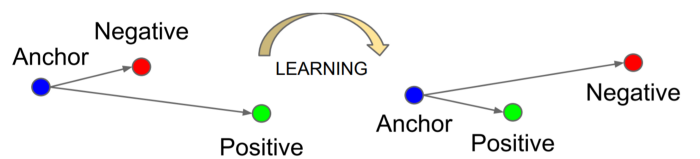
\includegraphics[width=\textwidth]{img/triplet_loss.png}
    \caption[Triplet loss]{The Triplet loss minimizes the distance between an anchor and a positive and maximizes the distance between the anchor and the negative datapoint.\\
    Source: \cite{tripletlossnn}}
    \label{fig:triplet_loss}
\end{figure}

This is the basic idea behind the triplet loss introduced by \cite{tripletlossfirst} and then further formalized by \cite{tripletlosssecond} and subsequently used as a loss function for \glspl{nn} by \cite{tripletlossnn}.

We shall use the triplet loss in following form:
\begin{defn}
Triplet loss for selected triplet (A, P, N) is:
\begin{equation}
\mathcal{L}(A, P, N) = \text{max}(\delta(f(A), f(P)) - \delta(f(A), f(N)) + \alpha, 0)
\label{eq:triplet}
\end{equation}
Where $f$ is a transformation given by \gls{nn}, $\delta$
is a selected distance function and $\alpha$ is a priori selected margin. The
selected triplet is a triplet of specific samples -- $A$ is a generic point
called ``anchor'' point, $P$ is a ``positive'' sample (i.e., sample of the same
cluster as anchor point) and $N$ is a ``negative'' sample (i.e., sample of
different cluster than anchor point).
\end{defn}


Such a definition provides the formula of the loss for a specific triplet. However, we can easily extend this notion by considering the average loss over all selected triplets.

It can be easily seen that the minimal value of the Triplet Loss is zero. In order to achieve this optimal value, not only do all ``in-between'' cluster distances have to be greater than ``within'' cluster distances, but they must be greater by at least a given margin $\alpha$.

\subsection{Triplet Selection}

An additional challenge for using Triplet Loss is to select suitable triplets. Usually, each point in the dataset (or more precisely in a subset of the dataset called a batch) is once selected as an anchor point. Then the task is to find the appropriate positive and negative sample for each anchor point.

The related terminology is somewhat ambiguous. For practical purposes, we choose to use the terminology corresponding to the implementation in the Tensorflow framework (\cite{tensorflow}). They operate with two strategies: Hard and Semi-Hard Triplet Loss.

In the case of Hard Loss, the positive and negative samples are selected ``as hard as possible'', which means that the positive sample is the furthest (from the anchor point) out of all considered samples of the same cluster. On the other hand, the negative sample is the closest sample out of all samples from samples that are not of the same cluster as the anchor point.

However, this intuitive selection of triplets can lead to bad local minima (\cite{tripletlossnn}). Therefore we also evaluate a different approach for triplet selection. The Semi-Hard approach selects such a pair of positive and negative samples that the negative sample is further away from the anchor point than the positive one, but not by the required margin. In terms of \autoref{eq:triplet} it means that $0 < \delta(f(A), f(N)) - \delta(f(A), f(P)) < \alpha$.